\documentclass[a4paper,notitlepage,11pt]{article}
\usepackage[dvipsnames]{xcolor}
\usepackage{tikz}
% add bulgarian support
\usepackage[utf8]{inputenc}
\usepackage[english,bulgarian]{babel}
\usepackage[T2B]{fontenc}
\usepackage[a4paper, total={7.5in, 10.5in}]{geometry}
\begin{document}
% turn off page numbering
\thispagestyle{empty}
Yordan Madzhunkov

\definecolor{myblue}{rgb}{0.0,0.7,1.0}
\definecolor{mylightblue}{rgb}{0.0,0.1,1.0}
\begin{figure}[t!]
  \hspace{-2cm}
%  \centering
\begin{tikzpicture}
   \coordinate (BL) at (-3,0);
   \coordinate (TR) at (19,3);

   \coordinate (A)  at (8,2.2);
   \coordinate (D)  at (8.8,3);

   \coordinate (A2) at (-3,2.2);
   \coordinate (B)  at (10.2,0);
   \coordinate (C)  at (11,0.8);
   \coordinate (C2) at (19,0.8);

%   \draw[step=1cm,gray,very thin] (BL) grid (TR);
   \draw[myblue, fill=myblue] (BL)--(B)--(A)--(A2)--cycle;
   \draw[myblue, fill=myblue] (C)--(D)--(TR)--(C2)--cycle;
   \draw[myblue, fill=myblue] (0,0.5) rectangle (2.7,3.5);
%   \draw[mylightblue, fill=mylightblue](A)--(B)--(C)--(D)--cycle;
%   \draw[myblue, fill=myblue] at (3.0, 0.0) rectangle (2.5cm, 3.0cm);
   \node[anchor=south west,inner sep=0] at (0.1,0.5) {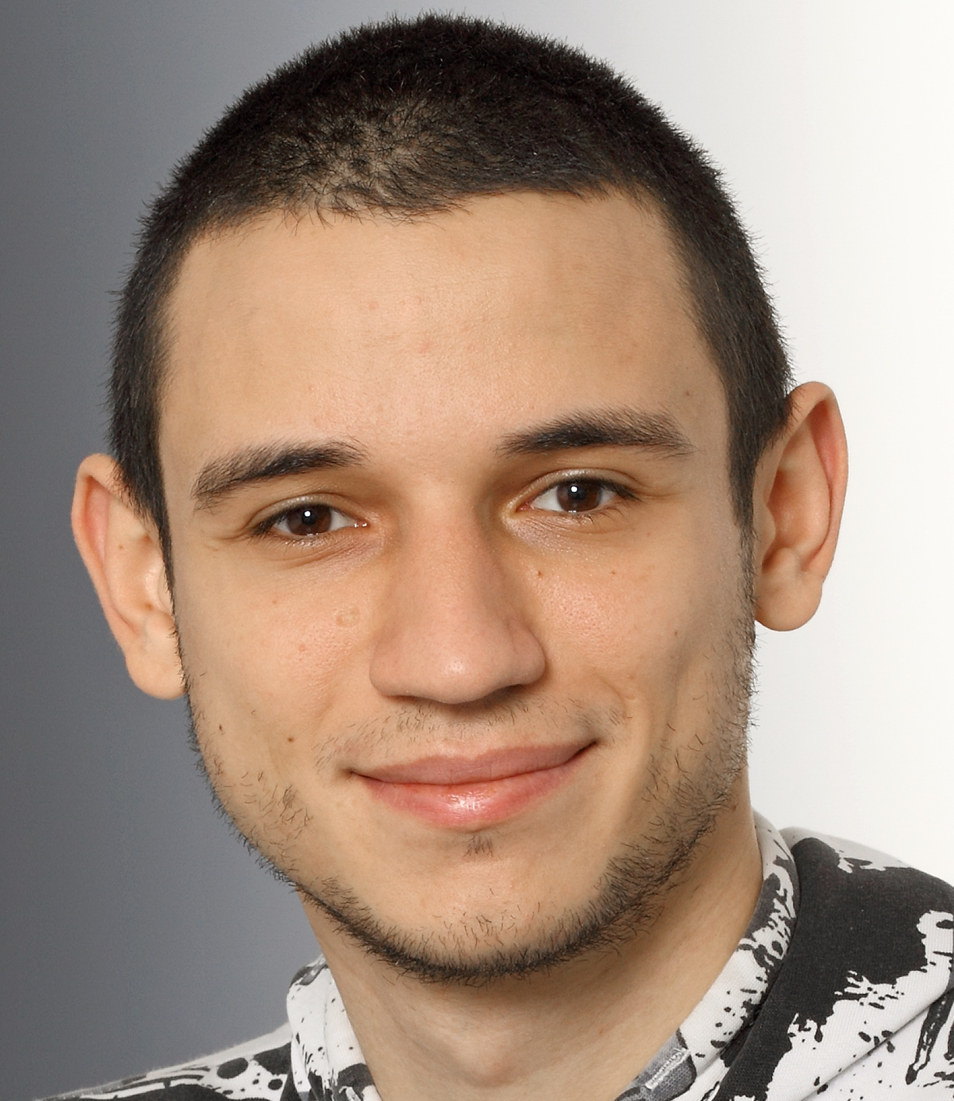
\includegraphics[width=2.5cm]{../ymadzhunkov.jpg}};
   \node[draw=none,align=left] at (6,1) {\color{white} \Large \textbf{Yordan Madzhunkov} \\ \color{white}Physicist, Software Developer};
\end{tikzpicture}
\end{figure}

%This will be useful later.
%\pagecolor{black}

\end{document}
